\documentclass{article}[18pt]
\ProvidesPackage{format}
%Page setup
\usepackage[utf8]{inputenc}
\usepackage[margin=0.7in]{geometry}
\usepackage{parselines} 
\usepackage[english]{babel}
\usepackage{fancyhdr}
\usepackage{titlesec}
\hyphenpenalty=10000

\pagestyle{fancy}
\fancyhf{}
\rhead{Sam Robbins}
\rfoot{Page \thepage}

%Characters
\usepackage{amsmath}
\usepackage{amssymb}
\usepackage{gensymb}
\newcommand{\R}{\mathbb{R}}

%Diagrams
\usepackage{pgfplots}
\usepackage{graphicx}
\usepackage{tabularx}
\usepackage{relsize}
\pgfplotsset{width=10cm,compat=1.9}
\usepackage{float}

%Length Setting
\titlespacing\section{0pt}{14pt plus 4pt minus 2pt}{0pt plus 2pt minus 2pt}
\newlength\tindent
\setlength{\tindent}{\parindent}
\setlength{\parindent}{0pt}
\renewcommand{\indent}{\hspace*{\tindent}}

%Programming Font
\usepackage{courier}
\usepackage{listings}
\usepackage{pxfonts}

%Lists
\usepackage{enumerate}
\usepackage{enumitem}

% Networks Macro
\usepackage{tikz}


% Commands for files converted using pandoc
\providecommand{\tightlist}{%
	\setlength{\itemsep}{0pt}\setlength{\parskip}{0pt}}
\usepackage{hyperref}

% Get nice commands for floor and ceil
\usepackage{mathtools}
\DeclarePairedDelimiter{\ceil}{\lceil}{\rceil}
\DeclarePairedDelimiter{\floor}{\lfloor}{\rfloor}

% Allow itemize to go up to 20 levels deep (just change the number if you need more you madman)
\usepackage{enumitem}
\setlistdepth{20}
\renewlist{itemize}{itemize}{20}

% initially, use dots for all levels
\setlist[itemize]{label=$\cdot$}

% customize the first 3 levels
\setlist[itemize,1]{label=\textbullet}
\setlist[itemize,2]{label=--}
\setlist[itemize,3]{label=*}

% Definition and Important Stuff
% Important stuff
\usepackage[framemethod=TikZ]{mdframed}

\newcounter{theo}[section]\setcounter{theo}{0}
\renewcommand{\thetheo}{\arabic{section}.\arabic{theo}}
\newenvironment{important}[1][]{%
	\refstepcounter{theo}%
	\ifstrempty{#1}%
	{\mdfsetup{%
			frametitle={%
				\tikz[baseline=(current bounding box.east),outer sep=0pt]
				\node[anchor=east,rectangle,fill=red!50]
				{\strut Important};}}
	}%
	{\mdfsetup{%
			frametitle={%
				\tikz[baseline=(current bounding box.east),outer sep=0pt]
				\node[anchor=east,rectangle,fill=red!50]
				{\strut Important:~#1};}}%
	}%
	\mdfsetup{innertopmargin=10pt,linecolor=red!50,%
		linewidth=2pt,topline=true,%
		frametitleaboveskip=\dimexpr-\ht\strutbox\relax
	}
	\begin{mdframed}[]\relax%
		\centering
		}{\end{mdframed}}



\newcounter{lem}[section]\setcounter{lem}{0}
\renewcommand{\thelem}{\arabic{section}.\arabic{lem}}
\newenvironment{defin}[1][]{%
	\refstepcounter{lem}%
	\ifstrempty{#1}%
	{\mdfsetup{%
			frametitle={%
				\tikz[baseline=(current bounding box.east),outer sep=0pt]
				\node[anchor=east,rectangle,fill=blue!20]
				{\strut Definition};}}
	}%
	{\mdfsetup{%
			frametitle={%
				\tikz[baseline=(current bounding box.east),outer sep=0pt]
				\node[anchor=east,rectangle,fill=blue!20]
				{\strut Definition:~#1};}}%
	}%
	\mdfsetup{innertopmargin=10pt,linecolor=blue!20,%
		linewidth=2pt,topline=true,%
		frametitleaboveskip=\dimexpr-\ht\strutbox\relax
	}
	\begin{mdframed}[]\relax%
		\centering
		}{\end{mdframed}}
\lhead{CSys}


\begin{document}
\begin{center}
\underline{\huge Memory}
\end{center}
\section{Memory}
\textbf{Goal:} Efficiently store large amount of data\\
3 common types:
\begin{itemize}
	\item DRAM
	\item SRAM
	\item ROM
\end{itemize}
M bit data stored at each N bit address
\begin{center}
	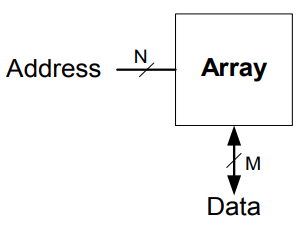
\includegraphics[scale=0.7]{memory}
\end{center}
\begin{itemize}
	\item 2 dimensional array of bit cells - each cell stores one bit
	\item N address bits and M data bits
	\begin{itemize}
		\item $2^N$ rows and M columns
		\item \textbf{Depth} - number of rows
		\item \textbf{Width} - number of columns
		\item \textbf{Array Size:} depth $\times$ width
	\end{itemize}
\end{itemize}
\begin{center}
	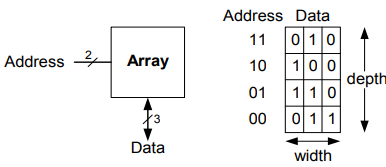
\includegraphics[scale=0.7]{memory1}
\end{center}
\subsection{Wordline}
\begin{itemize}
	\item A single row in memory array to be read/written
	\item Only one wordline high at once
\end{itemize}
\begin{center}
	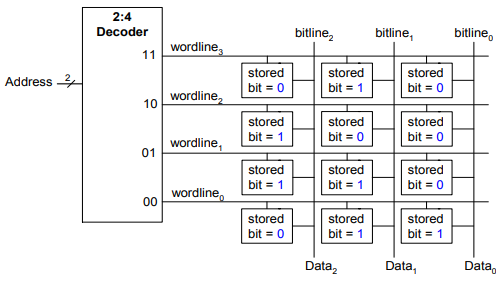
\includegraphics[scale=0.7]{wordline}
\end{center}
\begin{center}
	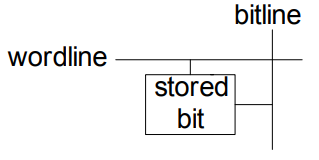
\includegraphics[scale=0.7]{wordline1}
\end{center}
On memory read:
\begin{itemize}
	\item If the wordline is active, the stored bit should drive the bitline value
	\item If the wordline is not active, the stored bit should not affect the bitline (leave it floating)
\end{itemize}
\subsection{Memory Diagrams}
\begin{center}
	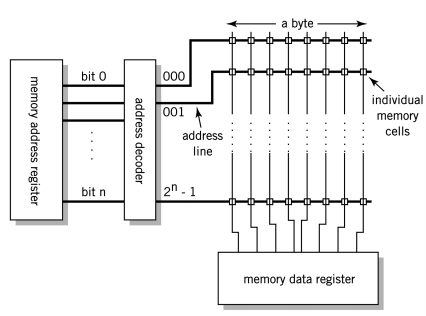
\includegraphics[scale=0.7]{memory_diagram}
\end{center}
\begin{center}
	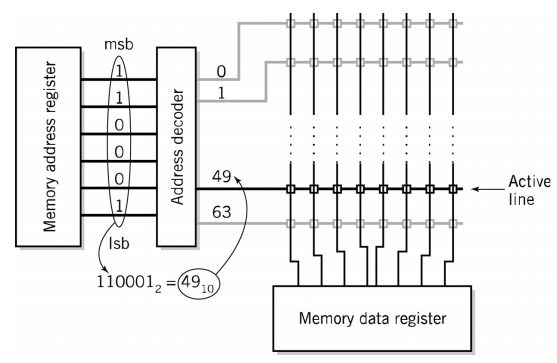
\includegraphics[scale=0.7]{memory_diagram1}
\end{center}
\begin{center}
	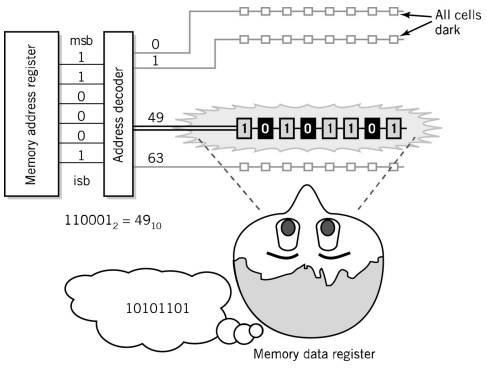
\includegraphics[scale=0.7]{memory_diagram2}
\end{center}
\subsection{Registers}
Memory consists of latches, each holding a single bit value, at an address\\
Interface between CPU and memory
\begin{itemize}
	\item MAR
	\item MDR
\end{itemize}
To speed access it is normal to address 8 bytes at a time, however the CPU can still isolate individual bytes when it needs to\\
\\
MAR holds the ‘open’ address, the CPU activates the group of bytes required - the address line \\
\\
MDR holds the activated data
\subsection{Lines}
Lines that control a memory cell
\begin{itemize}
	\item Wordline/ Address Line
	\begin{itemize}
		\item On when the computer is addressing the data in that cell
	\end{itemize}
	\item Read/Write Line
	\begin{itemize}
		\item Determines whether the data will be transferred to the MDR (write) or from the MDR (read) the cell 
	\end{itemize}
	\item Read occurs when
	\begin{itemize}
		\item Address line = 1 AND R/W line =1 
		\item Bitlines are left floating at the MDR, so take their values (weakly) from the active memory cells in the address line. 
	\end{itemize}
	\item Write occurs when
	\begin{itemize}
		\item Address line = 1 AND R/W line = 0 
		\item Bitlines are strongly driven by the MDR data, and overpower the weakly held bits in the active memory cells, overwriting the contents.
	\end{itemize}
\end{itemize}
\section{Types of memory}
Characteristics of the memory depend on the design of the individual cells:
\begin{itemize}
	\item RAM
	\begin{itemize}
		\item Originally named thus to distinguish from serial memory, e.g. magnetic tape
		\item Key feature: memory is volatile and is lost in power off.
		\item DRAM - dynamic RAM, dense but needs refreshing
		\item SRAM - static RAM less dense, but more stable.
	\end{itemize}
	\item ROM
	\begin{itemize}
		\item Originally was read only, and so named
		\item Key feature: memory persists even during power off
		\item Modern ROM memory, e.g. flash/SSD memory, can be written to
	\end{itemize}
\end{itemize}
\subsection{DRAM}
\begin{itemize}
	\item Each bit is one transistor and one capacitor. 
	\item The capacitor is charged or discharged to represent a bit. 
	\item Higher density, but slower.
	\item Capacitors discharge with time so need refreshing (reading and rewriting) every 64ms.
\end{itemize}
\begin{center}
	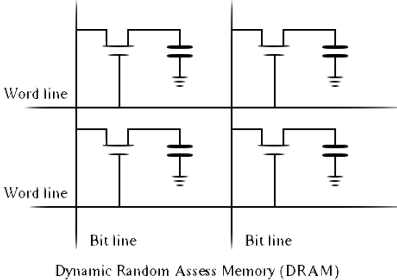
\includegraphics[scale=0.7]{DRAM}
\end{center}
\begin{itemize}
	\item Weakly driving the bitline as there is one capacitor driving the whole bitline
\end{itemize}
\subsection{SRAM}
\begin{itemize}
	\item 6 (or more) transistor flip-flop based memory
	\item Low density but stable and fast. 
	\item Doesn’t require refreshing but loses memory when powered off. 
	\item Can be easily incorporated into CPU manufacture
\end{itemize}
\begin{center}
	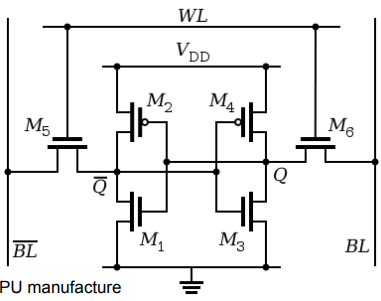
\includegraphics[scale=0.7]{SRAM}
\end{center}
\begin{center}
	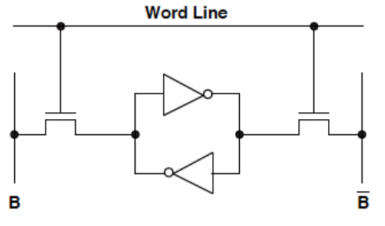
\includegraphics[scale=0.7]{SRAM1}
\end{center}
\begin{itemize}
	\item Activating wl and connecting lhs to bit value, B will give the driven value
	\item To write, send a strong signal to the not gates and they will flip into the opposite state
\end{itemize}
\subsection{ROM}
\subsubsection{Basic ROM}
\begin{itemize}
	\item To read the bitline is weakly set to high
	The wordline is then activated 
	\item If the cell contains a 0, the transistor
	connects the bitline to ground and the
	bitline goes low. 
	\item If the bitline contains a 1, the bitline retains
	the weak high it was initialised with.
\end{itemize}
\begin{center}
	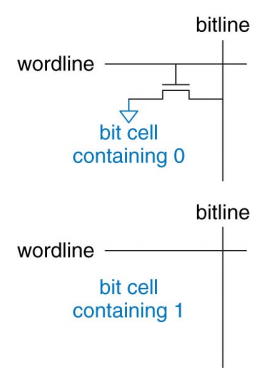
\includegraphics[scale=0.7]{basic_rom}
\end{center}
\subsubsection{Programmable ROM}
\begin{itemize}
	\item All bit cells have a transistor.
	By apply sufficient voltage a fuse can be blown
	to disconnect the transistors from ground in
	cells meant to contain 1s. 
	\item FLASH memory uses floating gate transistors
	instead, which can be electrically activated or
	deactivated. We won’t go into details.
\end{itemize}
\begin{center}
	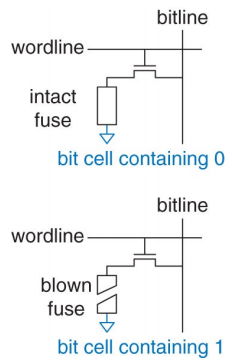
\includegraphics[scale=0.7]{PROM}
\end{center}
\section{Multi Ported Memory}
\begin{center}
	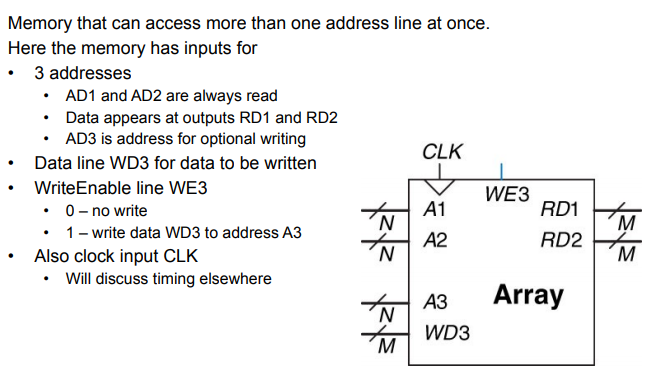
\includegraphics[scale=0.7]{multi-port}
\end{center}
\section{The MAR}
\begin{center}
	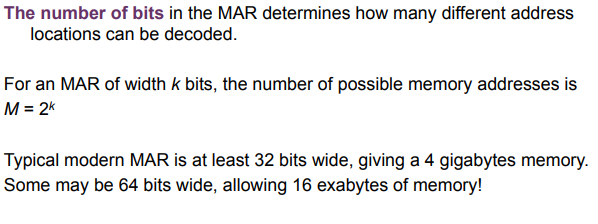
\includegraphics[scale=0.7]{MAR}
\end{center}
\section{Memory Hierarchy}
\begin{center}
	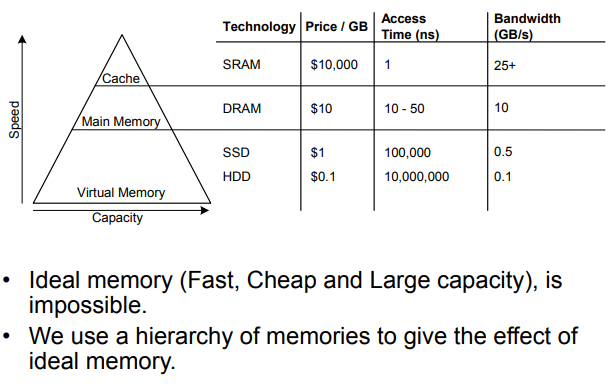
\includegraphics[scale=0.7]{heirarchy}
\end{center}
\section{Memory Speed}
\begin{center}
	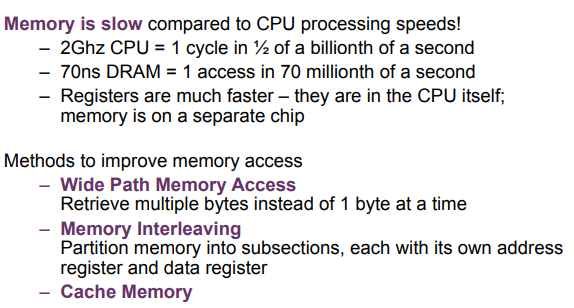
\includegraphics[scale=0.7]{soeed}
\end{center}
\section{Wide Path Memory Access}
\begin{center}
	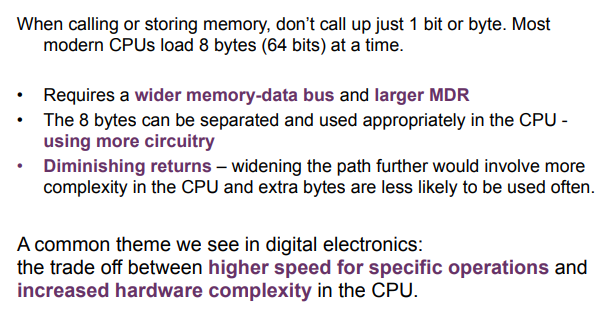
\includegraphics[scale=0.7]{wide-path}
\end{center}
\section{Memory Interleaving}
\begin{center}
	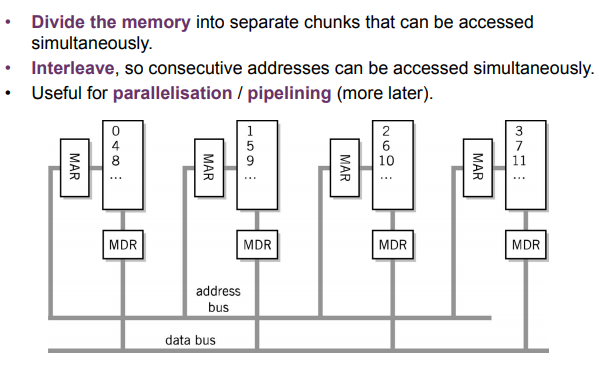
\includegraphics[scale=0.7]{interleaving}
\end{center}
\section{Cache Memory}
\begin{center}
	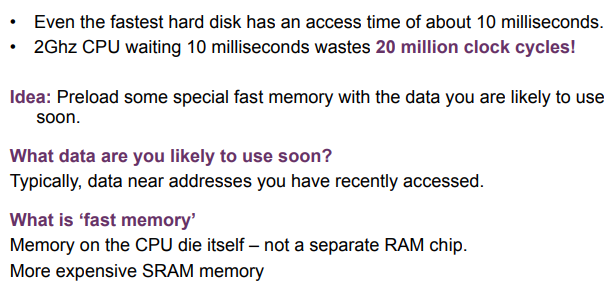
\includegraphics[scale=0.7]{cache}
\end{center}
\section{Locality}
\begin{center}
	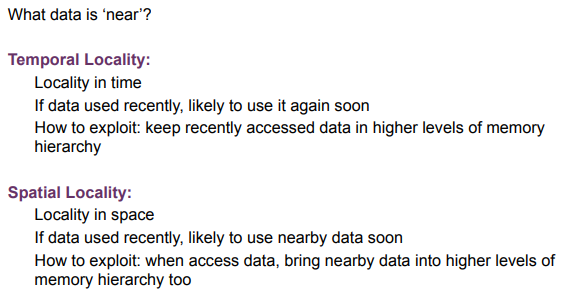
\includegraphics[scale=0.7]{locality}
\end{center}
\section{Cache Hit}
\begin{center}
	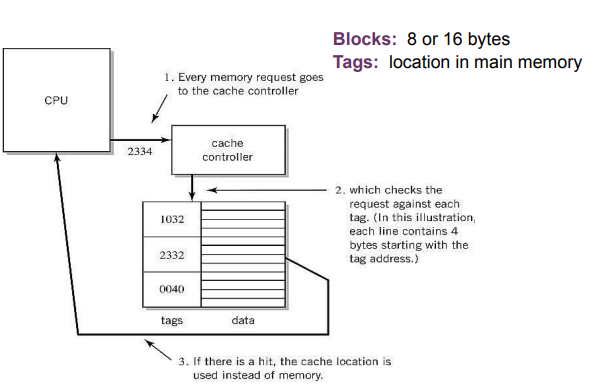
\includegraphics[scale=0.7]{cache-hit}
\end{center}
\section{Cache Miss}
\begin{center}
	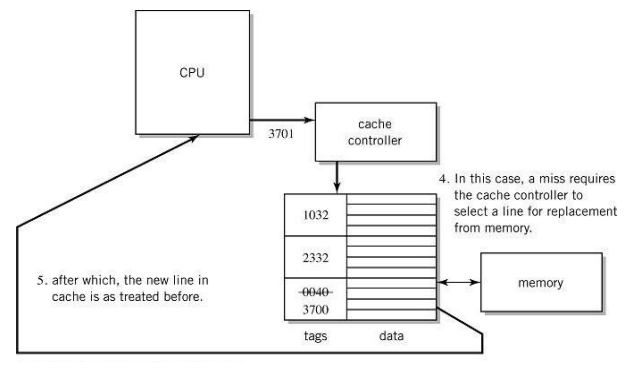
\includegraphics[scale=0.7]{cache-miss}
\end{center}
\section{Cache}
\begin{center}
	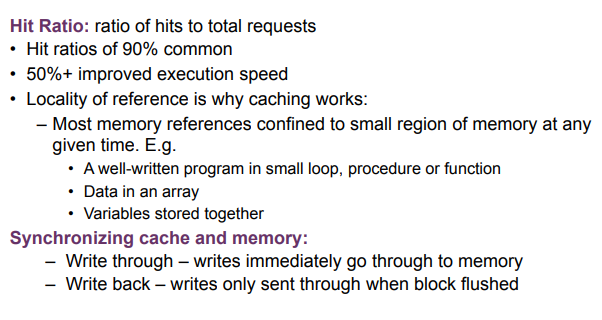
\includegraphics[scale=0.7]{cache1}
\end{center}
\section{Multi Level Cache}
\begin{center}
	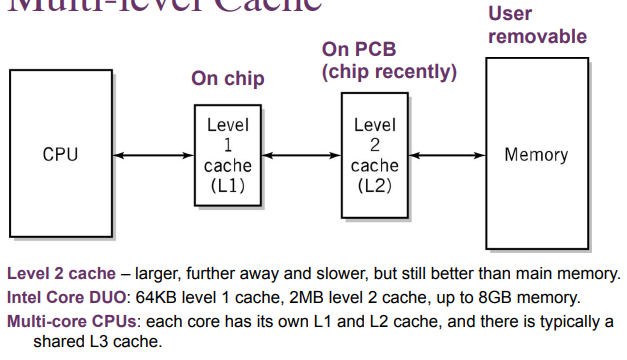
\includegraphics[scale=0.7]{multi-level-cache}
\end{center}


\end{document}